\documentclass[ 12pt, a4paper]{article}
\usepackage[ ]{indentfirst}
\usepackage[ ]{pdflscape}
\usepackage[ ]{graphicx}
\usepackage[ ]{booktabs}
\title{Revisão P1\\Construção de Compiladores\\Prof. Bráulio de Mello}
\author{Erickson G. Müller}
\date{23 de Abril de 2026}

\begin{document}
\maketitle
\section*{Conteúdos}
	\begin{itemize}
		\item Construção de Analisadores Léxicos
		\item Reconhecimento Sintático por APND
		\item APND, Analisador Sintático Preditivo
		\item Analisadores Left-Right
			\begin{itemize}
				\item Construção de tabela de parsing SLR
				\item Algoritmo de mapeamento do parser LR para análise sintática.
			\end{itemize}
	\end{itemize}
\newpage


\section{Construção de Analisador Léxico}

	A saída do Analisador Léxico é a entrada do Analisador Sintático.

\textbf{Processo:}
	\begin{enumerate}
		\item Definir tokens
		\item Construir o AFND
		\item Determinar o AF
		\item Acrescentar estado de erro para tratar tokens inválidos
		\item Construir o analisador (algoritmo)
		\item Tratamento de erro
		\begin{enumerate}
			\item Rótulo não reconhecido
			\item Descrição do erro
			\item Adicionar na Tabela de Símbolos
		\end{enumerate}
		\item Reconhecimento
	\end{enumerate}
	
	1 estado reconhece 1 token
	
	1 Token pode ser reconhecido por mais de 1 estado

	\subsection{Tabela de Símbolos}
		A tabela de símbolos segue a estrutura:
		
		\textit{Fita: [sequência de estados]+\$}
		
		\textit{L1: rótulo da cadeia}
		
		\textit{[Mensagem de erro]}
		
	\section{Reconhecedores Sintáticos}
	
		\begin{itemize}
			\item GLC
			\item Autômatos de PIlha
			\item APND
			\begin{itemize}
				\item $K$ - conjunto de estados
				\item $\sum$ - alfabeto de entrada
				\item $\Upsilon$ - alfabeto da pilha
				\item $\delta$ - função de transição (\textit{atua sobre a fita})
				\item $i$ - estado inicial ($i \in K$)
				\item $I$ - símbolo inicial da pilha ($I \in \Upsilon$)
				\item $F$ - conjunto de estados finais ($F \subseteq K$)
			\end{itemize}			
		\end{itemize}
		
		Se $(p, \alpha)\in \delta(q,a,Z)$ então $[q,ax,zy] \vdash^*[p,x,\alpha y]$.
		\textit{\\ 
		$^*$ $\vdash$ = transição/fecho transitivo\\ 
		$^*$ $\alpha$ = símbolo empilhamento\\
		$^*$ a = início da fita\\ 
		$^*$ Z = topo da pilha\\}
				
		\subsection{Aceitação por estado final}
			$L_{ef}(A)=\{ x \in \sum^* | [i,x,I] \vdash^* [f,\varepsilon,y]$ e $f\in F$ e $y \in \Upsilon^*$ qualquer$\}$
			
		\subsection{Aceitação por pilha vazia}
			$L_{pv}(A)=\{ x \in \sum^* | [i,x,I] \vdash^* [f,\varepsilon,\varepsilon]$ e $f\in K$ qualquer$\}$
			
		\subsection{Exemplo}
			$K = \{0,1,2\}$
			
			$i = {0}$
			
			$\sum = \{a,b\}$
			
			$I=X$
			
			$\Upsilon = \{X,A\}$
			
			$F=\{2$\}
			
%			\textbf{
\textbf{Funções de Transição}

				$$1: \delta(0,a,X)=\{(0,AX)\}$$
				$$2: \delta(0,a,A)=\{(0,AA)\}$$
				$$3: \delta(0,b,A)=\{(1,\varepsilon)\}$$
				$$4: \delta(1,b,A)=\{(1,\varepsilon)\}$$
				$$5: \delta(1,\varepsilon,X)=\{(2,X)\}$$
				
%			}
Fita Resultada do analisador léxico:

\textit{Fita:} $[0,aaabbb,X]\vdash$

* \textit{Lembrar que estado inicial é 0 e X está no topo da pilha.}

1ª transição: $[0,aaabbb,X]\vdash [0,aabbb,AX]$

2ª transição: $[0,aaabbb,X]\vdash [0,aabbb,AX] \vdash [0,abbb,AAX]$

3ª transição: $[0,aaabbb,X]\vdash [0,aabbb,AX] \vdash [0,abbb,AAX] \vdash [0,bbb,AAAX]$

4ª transição: $[0,aaabbb,X]\vdash [0,aabbb,AX] \vdash [0,abbb,AAX] \vdash [0,bbb,AAAX] \vdash [1,bb,AAX]$

5ª transição: $[0,aaabbb,X]\vdash [0,aabbb,AX] \vdash [0,abbb,AAX] \vdash [0,bbb,AAAX] \vdash [1,bb,AAX] \vdash [1,b,AX]$

6ª transição: $[0,aaabbb,X]\vdash [0,aabbb,AX] \vdash [0,abbb,AAX] \vdash [0,bbb,AAAX] \vdash [1,bb,AAX] \vdash [1,b,AX] \vdash [1,\varepsilon, X] $

7ª transição: $[0,aaabbb,X]\vdash [0,aabbb,AX] \vdash [0,abbb,AAX] \vdash [0,bbb,AAAX] \vdash [1,bb,AAX] \vdash [1,b,AX] \vdash [1,\varepsilon, X] \vdash [2,\varepsilon, X]$

Assim, $[2,\varepsilon,X] \in F$

		\subsection{Exemplo 2}
		
			$K=\{0,1\}$
			
			$i= \{0\}$
			
			$\sum = \{a,b\}$
			
			$I=\{X\}$
			
			$\Upsilon = \{X,A\}$
			
			$F = \O$
			
			\textbf{Funções de Transição}
			
			$$1:\delta(0,a,X) = \{(0,A)\}$$
			$$2:\delta(0,a,A) = \{(0,AA)\}$$
			$$3:\delta(0,b,a)= \{(1,\varepsilon)\}$$
			$$4:\delta(1,b,A)=\{(1,\varepsilon)\}$$
			
			\textit{Fita:} $[0,aabbb,X]\vdash [0,abbb,A] \vdash [0,bbb,AA] \vdash [1,bb,A] \vdash [1,b,\varepsilon]$ \textbf{não ocorreu reconhecimento no último estado}
			
		\subsection{Exemplo Gramática de Operadores}
		
			$E::= E+T | T$
			
			$T::= T*F | F$
			
			$F::= (E) | a$
			
			Reconhecimento por pilha vazia
			
			\textit{Fita:}$[0,a*(a+a),E]\vdash$
			
			\textbf{Criação de regras:}
			$$1: \delta(0,\varepsilon, E) = \{(0,T)\}$$
			\textit{Comentário: o autômato de pilha é não determinístico pois não podemos escolher qual produção da regra será usado na transição para reduzir e acrescentar no topo da pilha. A regra 1 reduz uma produção de E e empilha uma produção de T}
			
			\textit{Fita:}$[0,a*(a+a),E]\vdash [0,a*(0+a),T] \vdash$
			
			\textbf{Criação de nova regra:}
			$$1: \delta(0,\varepsilon, E) = \{(0,T)\}$$
			$$2: \delta(0,\varepsilon,T) = \{(0,T*F),(0,F)\}$$
			
			\textit{Fita:}$[0,a*(a+a),E]\vdash [0,a*(0+a),T] \vdash [0,a*(a+a),T*F] \vdash [0,a*(a+a), F*F] \vdash$
			
			\textbf{Criação de nova regra:}
			\textbf{Criação de nova regra:}
			$$1: \delta(0,\varepsilon, E) = \{(0,T)\}$$
			$$2: \delta(0,\varepsilon,T) = \{(0,T*F),(0,F)\}$$
			$$3:\delta(0,\varepsilon,F)=\{(0,a)\}$$
			$$4:\delta(0,a,a)=\{(0,\varepsilon)\}$$
			
			\textit{Fita:}$[0,a*(a+a),E]\vdash [0,a*(0+a),T] \vdash [0,a*(a+a),T*F] \vdash [0,a*(a+a), F*F] \vdash [0,a*(a+a), a*F] \vdash [0,*(a+a),*F] \vdash [0,(a+a),F] \vdash [0,(a+a),(E)] \vdash$
			
			\textbf{Criação de novas funções:}
			$$1: \delta(0,\varepsilon, E) = \{(0,T)\}$$
			$$2: \delta(0,\varepsilon,T) = \{(0,T*F),(0,F)\}$$
			$$3:\delta(0,\varepsilon,F)=\{(0,a)\}$$
			$$4:\delta(0,a,a)=\{(0,\varepsilon)\}$$
			$$5:\delta(0,*,*)=\{(0,\varepsilon)\}$$
			$$6:\delta(0,(,()=\{(0,\varepsilon)\}$$
			
			\textit{Fita:}$[0,a*(a+a),E]\vdash [0,a*(0+a),T] \vdash [0,a*(a+a),T*F] \vdash [0,a*(a+a), F*F] \vdash [0,a*(a+a), a*F] \vdash [0,*(a+a),*F] \vdash [0,(a+a),F] \vdash [0,(a+a),(E)] \vdash [0, a+a), E)] \vdash [0, a+a) , E+T)] \vdash [0,a+a, T+T)] \vdash [0,a+a),F+T)]\vdash [0,a+a),a+T)] \vdash [0, +a), +T)] \vdash$
			
			\textbf{Criação da regra para + no inicio da fita e + no topo da pilha:}
			$$1: \delta(0,\varepsilon, E) = \{(0,T)\}$$
			$$2: \delta(0,\varepsilon,T) = \{(0,T*F),(0,F)\}$$
			$$3:\delta(0,\varepsilon,F)=\{(0,a)\}$$
			$$4:\delta(0,a,a)=\{(0,\varepsilon)\}$$
			$$5:\delta(0,*,*)=\{(0,\varepsilon)\}$$
			$$6:\delta(0,(,()=\{(0,\varepsilon)\}$$
			$$7:\delta(0,+,+)= \{(0,\varepsilon)\}$$
			
			\textit{Fita:}$[0,a*(a+a),E]\vdash [0,a*(0+a),T] \vdash [0,a*(a+a),T*F] \vdash [0,a*(a+a), F*F] \vdash [0,a*(a+a), a*F] \vdash [0,*(a+a),*F] \vdash [0,(a+a),F] \vdash [0,(a+a),(E)] \vdash [0, a+a), E)] \vdash [0, a+a) , E+T)] \vdash [0,a+a, T+T)] \vdash [0,a+a),F+T)]\vdash [0,a+a),a+T)] \vdash [0, +a), +T)] \vdash [0,a),T)] \vdash [0,a),F)] \vdash [0,a),a)] \vdash [0,),)] \vdash$
			
			\textbf{Criação de nova regra:}
			
			$$1: \delta(0,\varepsilon, E) = \{(0,T),(0,E+T)\}$$
			*\textit{em algum momento foi adicionado }
			$$2: \delta(0,\varepsilon,T) = \{(0,T*F),(0,F)\}$$
			$$3:\delta(0,\varepsilon,F)=\{(0,a),(0,(E)\}$$
			*\textit{em algum momento foi adicionado}
			$$4:\delta(0,a,a)=\{(0,\varepsilon)\}$$
			$$5:\delta(0,*,*)=\{(0,\varepsilon)\}$$
			$$6:\delta(0,(,()=\{(0,\varepsilon)\}$$
			$$7:\delta(0,+,+)= \{(0,\varepsilon)\}$$
			$$8:\delta(0,),))= \{(0,\varepsilon)\}$$
			
			\textit{Fita:}$[0,a*(a+a),E]\vdash [0,a*(0+a),T] \vdash [0,a*(a+a),T*F] \vdash [0,a*(a+a), F*F] \vdash [0,a*(a+a), a*F] \vdash [0,*(a+a),*F] \vdash [0,(a+a),F] \vdash [0,(a+a),(E)] \vdash [0, a+a), E)] \vdash [0, a+a) , E+T)] \vdash [0,a+a, T+T)] \vdash [0,a+a),F+T)]\vdash [0,a+a),a+T)] \vdash [0, +a), +T)] \vdash [0,a),T)] \vdash [0,a),F)] \vdash [0,a),a)] \vdash [0,),)] \vdash [0,\varepsilon, \varepsilon \vdash ^*$
			
			
		\section{Tarefa com a mesma gramática}
			\textbf{Fita:}\\
			$[0,a*((a+(a*a)),E] \vdash$
			\\
		\subsection{Tarefa: montar o conjunto de funções de transição}		
			\textbf{Gramática}\\
			$S::=<A> <S>|\varepsilon$\\
			$A::=$ se $cond$ então $<B> |$ enquanto $cond \{<C>\}$\\
			$B::= \{<C>\} | \{<C>\} $ else $\{<C>\}$\\			
			$C::= <A> |$ exp\\
			
	\newpage
	\section{Análise Preditiva Tabular}
		O analisador preditivo precisa do conjunto \textit{follow}, por isso usamos o símbolo de final de sentença. X = topo da pilha. N = conjunto dos não terminais. Quando aparecer um V maiúsculo é um terminal v (OR).
		\\
		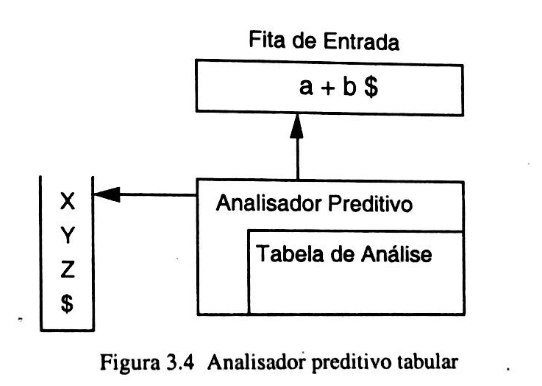
\includegraphics[scale=0.8]{images/analisador.png}
		
		\begin{enumerate}
			\item se $X = a = \$ $, aceita
			\item se $X = a \neq \$$
			\begin{itemize}
				\item desempilha $a$
				\item avança posição de leitura na fita
			\end{itemize}
			\item se $X \in N$
			\begin{itemize}
				\item consulta $M[X,a]$
				\item se $M[X,a] = \{X::=UVW\}$
				\item se $M[X,a] = \o$, erro
			\end{itemize}
		\end{enumerate}
		\begin{center}
		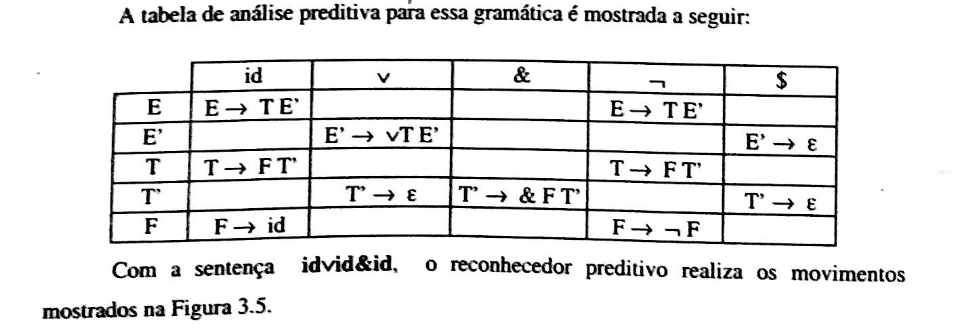
\includegraphics[scale=0.65]{images/tabela.png}
		
		\textit{substituir id por a}
		\end{center}
		$E::= EvT | T$\\
		$T::= T\&F | F$\\
		$F::= \neg F | a$
		\\
		O analisador preditivo não reconhece recursão à esquerda, portanto vamos retirar a recursão.
		\\
		$E::= TE'$\\
		$E'::= VTE' | \varepsilon$\\
		$T::=FT'$\\
		$T'::= \&FT'| \varepsilon$\\
		$F::=\neg F | a$\\
		Essa gramática é recursiva à direita e não à esquerda. \\ \\		
		\\
		o inicio do topo da pilha é definido pelo símbolo inicial da gramática.\\
		\begin{tabular}{|c|c|c|}
			Pilha $E\$ $ & Entrada da fita & ação \\
			$\$TE' \$$ & $a v a \& a \$$ & $E::=TE'$\\
			$FT'E'\$$ & $ava\&a\$ $ & $T::=FT'$ \\
			$aT'E' \$ $ & $ava\&a \$ $ & $F::a$ \\
			$T'E' \$ $ & $va\&a\$ $ & $T'::\varepsilon$\\
			$E'\$ $ & $va\&a\$ $ & $E' ::= VTE'$\\
			$VTE'\$ $ & $va\& a \$ $ & $T'::=FT'$\\
			$TE' \$ $ & $a\& a \$ $ & \\
			$FT'E'\$ $ & $a\&a\$ $ & $F::= a$\\  
			$aT'E'\$ $ & $a\&a\$ $& $T'::=\&FT'$\\
			$T'E'\$$ & $\&a\$ $ & \\
			$\&FT'E'\$ $ & $\&a\$ $ & $T'::= \&FT' $\\
%			$\&FT'E'\$$ & $\&a\$ $ & \\
			$FT'E'\$ $ & $a\$ $ & $F::=a$\\
			$aT'E'\$ $ &$a\$ $ \\
%			$aT'E'\$ $& $\$ $ & \\
			$T'E'\$ $ &  $\$ $ & $T'::=\varepsilon$\\
			$E'\$ $ & $\$ $& $E'::\varepsilon$\\
			$\$$ & $\$ $ &  Aceite\\ 
			
		
		\end{tabular}
		\\ \\ Tabela first e follow:: \\
		\begin{tabular}{|c|c|c|}
				& First 		& Follow		\\
			E	& $\neg , a $ 		& $\$			$\\
			E'	& $V,\varepsilon$	& $\$			$\\
			T	& $\neg, a $		& $V, \$		$\\
			T'	& $\&, \varepsilon$	& $V, \$		$\\
			F	& $ \neg, a $		& $\&,V, \$		$\\
		
		\end{tabular}
		
		Para acrescentar uma ação na tabela preditiva, a produção será acrescentada na linha definida pelo símbolo que dá nome à regra nas colunas do first da produção. Quando uma produção é $\varepsilon$, acrescentamos a produção na linha do símbolo que dá nome à regra nas colunas definidas pelo follow do mesmo símbolo. 
		
		\subsection{Tarefa com a gramática do TF1}
			\textbf{Gramática}\\
			$S::= AS|\varepsilon$\\
			$A::=$ se $cond$ então $B |$ enquanto $cond \{C\}$\\
			$B::= \{C\} | \{C\} $ senao $\{C\}$\\			
			$C::= A |$ exp\\
			
			\textbf{Eliminação da recursão à esquerda}:
			Não existe nenhuma recursão à esquerda nessa gramática.
			
			\textbf{Construção da tabela de análise preditiva:}
			
\begin{landscape}
	
	\textbf{Gramática Fatorada:}\\
	$S::= AS|\varepsilon$\\
	$A::=$ se $cond$ então $B |$ enquanto $cond \{C\}$\\
	$B::= \{C\}B'$\\
	$B'::=$ senao $\{C\} | \varepsilon $\\			
	$C::= A |$ exp\\
\thispagestyle{empty}
\begin{table}[h]
\centering
\makebox[\textwidth][c]{
\begin{tabular}{|c|c|c|c|c|c|c|c|c|c|}

\toprule
&$ se			$&$ cond	$&$ entao	$&$ enquanto	$&$ 	\{	$&$	\}	$&$ senao	$&$ exp		$&$ \$			$\\
\hline
$S$&$ S\to AS		  	$&$		$&$		$&$ S\to AS	$&$		$&$		$&$		$&$		$&$ S\to \varepsilon 	$\\
\hline
$A$&$  A\to $se cond entao $B  	$&$		$&$		$&$ A\to $ enquanto cond $\{C\}		$&$		$&$		$&$		$&$		$&$		$\\
\hline
$B$&$     			$&$		$&$		$&$		$&$ B\to \{C\}B'	$&$		$&$		$&$		$&$		$\\
\hline
$B'$&$ B' \to \varepsilon     			$&$		$&$		$&$ B' \to \varepsilon		$&$ 			$&$  B' \to \varepsilon		$&$ B'\to$ senao $\{C\}		$&$		$&$ B' \to \varepsilon	$\\
\hline
$C$&$ C\to A   			$&$		$&$		$&$ C\to A	$&$		$&$		$&$		$&$ C\to exp	$&$		$\\
\bottomrule
			
\end{tabular}
}
\end{table}
\end{landscape}

\section{Analisadores LR}
	\begin{itemize}
		\item redutores (ascendentes)
		\item esquerda $\to$ direita (\textbf{derivação} mais à direita)
		\item estruturas sintáticas LLC
		\item identificação de erros (lookahead LALR)
		\item exige mais esforço de implementação
		\item SLR
		\item LALR (precisa adicionar a transição da próxima transição e da seguinte)
		\item LR
		\item utiliza a pilha
	\end{itemize}
	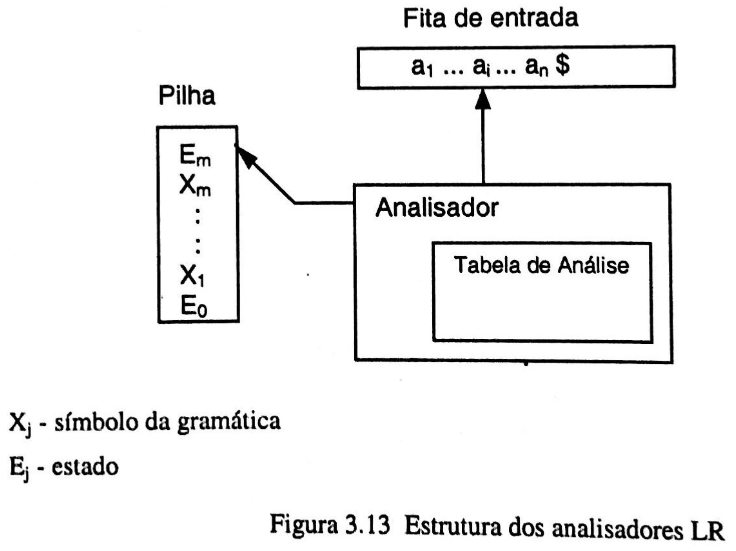
\includegraphics[scale=0.6]{images/analisador_lr.png}

	\subsection{Ações da tabela de análise}
		\begin{itemize}
			\item Empilha
			\item Reduz (sempre é seguida por um salto)
			\item Salto
			\item Aceite (reconhecimento e acontece em uma situação só da tabela)
			\item Erro (identificação e tratamento)
		\end{itemize}

	\subsection{Passos de construção de um analisador LR}
		\begin{itemize}
			\item GLC
			\item Itens válidos (canônicos)
			\item Transições pelos terminais (from itens válidos)
			\item Saltos pelos não-terminais, depois de uma redução(from itens válidos)
			\item First/Follow
			\item Construção da Tabela de Análise a partir de:
				\begin{enumerate}
					\item Estados
					\item Transições
					\item Saltos
					\item Follow
					\item Identificador das produções
				\end{enumerate}
			\item Algoritmo de reconhecimento
			\item ID das produções
		\end{itemize}
	\subsection{Construção do conjunto de itens válidos:}

		$S::= a|[L]$

		$L::= L;S | S$

		Iniciar pelo estado 0. \textit{Todas as produções do estado inicial precisam aparecer no estado 0}

		$Io =\{$\\
		Itens válidos:\\
		$S'::=S\$$\\
		$S::= a|[L]$\\
		$L::= L;S | S$\\
		$I_0 =\{S'::=\bullet S\$, S::=\bullet a,S::=\bullet [L]\}$\\
		$S'\to \bullet $\\
		\textbf{1-Transição pelo mesmo Sb no estado de origem?}\\
		\textbf{2-Estado corrente ($\bullet$) precede um NT? Se não, não precisa copiar as regras desse não terminal}\\
		$I_1 =\{S'::=S\bullet \$\}(Completo!)$\\
		$I_2 =\{S::=a\bullet \}(Completo!)$\\
		\textbf{3-Estado Corrente ($\bullet$) está no final de algum item válido(produção)? Se sim, esse estado possui um item chamado de "completo" que vai resultar numa ação de redução seguida de um salto.}\\
		$I_3 =\{S::=[\bullet L], L::= \bullet L;S, L::=\bullet S, S::=\bullet a, S::=\bullet [L] \}$\\
		$I_4 =\{S::=[L\bullet],L::=L\bullet ;S\}$\\
		$I_5 = \{ L::=S\bullet\}(Completo!)$\\
		$I_6 = \{ S::= [L]\bullet\}(Completo!)$\\
		$I_7 = \{ L::= L;\bullet S, S::= \bullet a, S::= \bullet [L] \}$\\
		$I_8 = \{ L::= L;S \bullet\} $ (Completo!)\\
	\subsection{Construção das transições:}
		Partindo de um estado, olhar para o item e o estado corrente dele e identificar o estado em que o item tenha transição. Quando a transição ocorre com um símbolo não terminal, temos um salto, quando é por um terminal, temos um empilhamento.\\
		$T(I_0,S)=I_1$\\
		$T(I_0,a)=I_2$\\
		$T(I_0,[)=I_3$\\
		$T(I_3,L)=I_4$\\
		$T(I_3,S)=I_5$\\
		$T(I_3,a)=I_2$\\
		$T(I_3,[)=I_3$\\
		$T(I_4,])=I_6$\\
		$T(I_4,;)=I_7$\\
		$T(I_7,S)=I_8$\\
		$T(I_7,a)=I_2$\\
		$T(I_7,[)=I_3$\\
	%\subsection{Construção dos saltos:}
\newpage
\section{Construir conjunto de itens válidos, transições e saltos}
	\textbf{Gramática:}\\
	$E::=E+T| \bullet T$\\
	$T::=T*F|F$\\
	$F::= (E) | a $\\
	$I_0 = \{ E' ::= \bullet E \$ , E::= \bullet E+T, E::= \bullet T, T::= \bullet T*F, T::= \bullet F, F::= \bullet (E), F::= \bullet a \}$\\
	$I_1 = \{E' ::= E \bullet \$, E::= E\bullet +T \}  $ \\
	$I_2 = \{E::= T\bullet, T::= T\bullet *F\}  $ (Completo) \\
	$I_3 = \{T::= F \bullet \}  $ (Completo) \\
	$I_4 = \{F::= (\bullet E), E::= \bullet E+T, E::= \bullet T, T::= \bullet T * F, T::= \bullet F, F::= \bullet (E), F::= \bullet a\}  $ \\
	$I_5 = \{F::= a\bullet\}  $ (Completo) \\
	$I_6 = \{E::= E+\bullet T, T::= \bullet T*F, T::= \bullet F, F::= \bullet(E), F::= \bullet a\}  $ \\
	$I_7 = \{T::= T*\bullet F,F::= \bullet(E), F::= \bullet a\}$ \\
	$I_8 = \{F::= (E\bullet), E::= E \bullet + T\}  $ \\
	$I_9 = \{E::= E+T \bullet, T::= T\bullet * F,   $ (Completo) \\
	$I_{10} = \{T::= T*F \bullet\}  $ (Completo) \\
	$I_{11} = \{F::= (E)\bullet\}  $ (Completo)\\

\section{Construção da Tabela SLR}
	Para construir a Tabela SLR precisamos do conjunto de transições, conjunto de saltos, conjunto First e conjunto Follow.

	\textbf{Gramática:}\\
	$E'::E\$$\\
	$E::=E+T| \bullet T$\\
	$T::=T*F|F$\\
	$F::= (E) | a $\\
		 Tabela first e follow: \\
\begin{tabular}{|c|c|c|}
	& First 		& Follow			\\
E	& $ (, a	$	& $\$,+,)		$\\
T	& $ (, a	$	& $ *, \$, +, )		$\\
F	& $ (, a	$	& $ *, \$, +, )		$\\
	
\end{tabular}\\
	Conjunto de Transições e Saltos:\\
	$T(I_0,E)=I_1, T(I_0)= I_2, T(I_0,F) = I_3, T(I_0, ()=I_4, T(I_0,a)=I_5$\\
	$T(I_1,+)= I_6$\\
	$T(I_2,*)=I_7$\\
	$T(I_4, *) = I_8, T(4,T)=I_2, T(I_4,F) = I_3, T(I_4,()=I_4, T(I_4,a)=I_5$\\
	$T(I_6,T)=I_9,T(I_6,F)=I_3,T(I_6,()=I_4,T(I_7,a)=I_5$\\
	$T(I_7,F) = I_{10}, T(I_7,()=I_4, T(I_7,a)= I_5$\\
	$T(I_8,)) = I_{11}, T(I_8, +) = I_6$\\
	$T(I_9,*)=I_7$\\

	Tabela sem operações de redução\\
	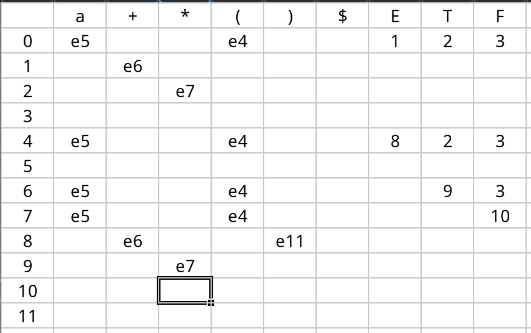
\includegraphics{images/tabela_SLR.png}
	A operação de redução é apenas para o item completo. Para o estado 2, para $E::T$, nós vamos adicionar na tabela a Redução. Lembrando que o número da redução é referente à ordem das produções da gramática.

\begin{verbatim}
para I2
		para E::=T
		add R2
		linha 2
		colunas do Follow (E)


para I3
	para
	add R4
	coluna do Follow (T)
\end{verbatim}

	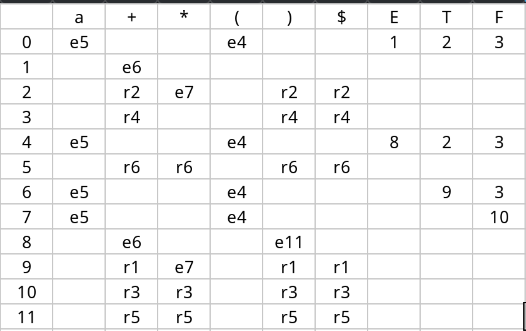
\includegraphics{images/tabela_SLR_completa.png}\\
	Incluir Aceite no final de sentença\\
	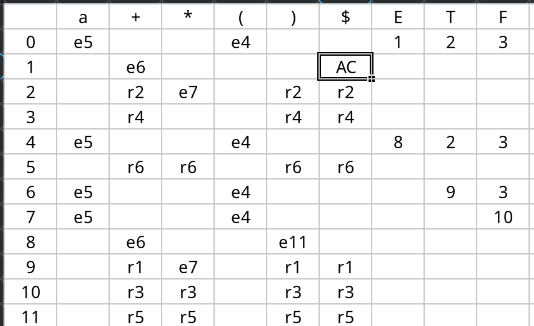
\includegraphics{images/tabela_SLR_aceite.png}

\newpage
\begin{verbatim}
0						a * a + a $ 					(e5)
a5						* a + a $				 	(r6)
0											(reduz 2)
0F											(salto)
0F3						* a + a $					(r4)
0											(reduz 2)
0T											(salto)
0T2	
0T2*7						a + a $	
0T2*7a5						+ a $				 (r6)
0T2*7											(reduz 2)
0T2*7F											(salto)
0T2*7F10					+ a $				 (r3)
...						...
0T2						+ a $				 (r2)
...						...
0E1						+ a $				 (e6)
0E1+6						a $				 (e5)
0E1+6a5						$				 (r6)
0E1+6F3						$				 (r4)
0E1+6T9						$				 (r1) % reduz sempre o dobro
0						$
0E1						AC

\end{verbatim}
\section{Construir a tabela SLR}

	\textbf{Gramática}\\
	$S::=<A> <S>|\varepsilon$\\
	$A::=$ se $cond$ então $<B> |$ enquanto $cond \{<C>\}$\\
	$B::= \{<C>\} | \{<C>\} $ else $\{<C>\}$\\			
	$C::= <A> |$ exp\\

\newpage
\section{Construir a tabela SLR}
	Gramática\\
	$S::=$ enq opl faça $\{A\}$ | se opl então $\{A\}$\\
	$A::=$ $S$ | exp\\
Reconhecer cadeia:
	Conjunto de Transições e Saltos:\\
	$T(I_0,E)=I_1, T(I_0)= I_2, T(I_0,F) = I_3, T(I_0, ()=I_4, T(I_0,a)=I_5$\\
	$T(I_1,+)= I_6$\\
	$T(I_2,*)=I_7$\\
	$T(I_4, *) = I_8, T(4,T)=I_2, T(I_4,F) = I_3, T(I_4,()=I_4, T(I_4,a)=I_5$\\
	$T(I_6,T)=I_9,T(I_6,F)=I_3,T(I_6,()=I_4,T(I_7,a)=I_5$\\
	$T(I_7,F) = I_{10}, T(I_7,()=I_4, T(I_7,a)= I_5$\\
	$T(I_8,)) = I_{11}, T(I_8, +) = I_6$\\
	$T(I_9,*)=I_7$\\

	Tabela sem operações de redução\\
	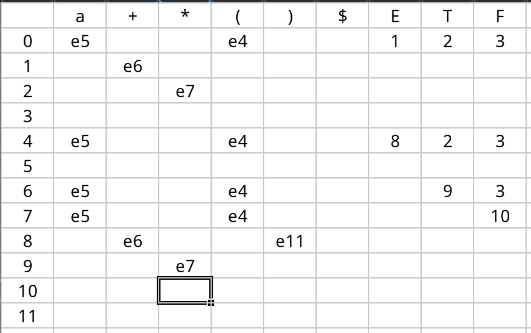
\includegraphics{images/tabela_SLR.png}
	A operação de redução é apenas para o item completo. Para o estado 2, para $E::T$, nós vamos adicionar na tabela a Redução. Lembrando que o número da redução é referente à ordem das produções da gramática.

\begin{verbatim}
para I2
		para E::=T
		add R2
		linha 2
		colunas do Follow (E)


para I3
	para
	add R4
	coluna do Follow (T)
\end{verbatim}

	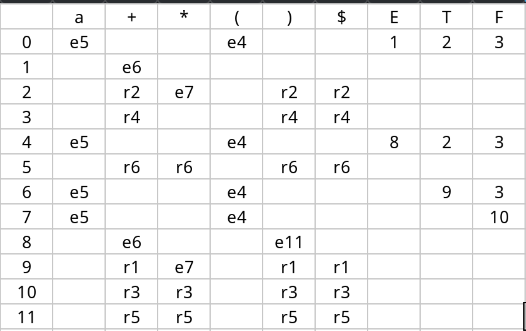
\includegraphics{images/tabela_SLR_completa.png}\\
	Incluir Aceite no final de sentença\\
	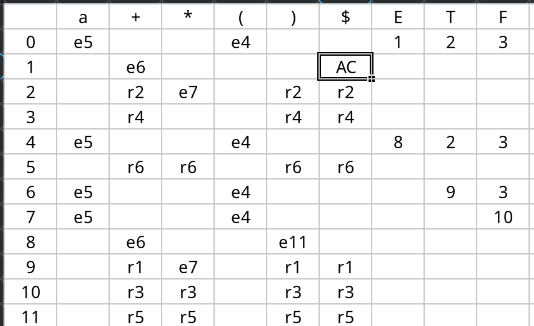
\includegraphics{images/tabela_SLR_aceite.png}

\newpage
\begin{verbatim}
0						a * a + a $ 					(e5)
a5						* a + a $				 	(r6)
0											(reduz 2)
0F											(salto)
0F3						* a + a $					(r4)
0											(reduz 2)
0T											(salto)
0T2	
0T2*7						a + a $	
0T2*7a5						+ a $				 (r6)
0T2*7											(reduz 2)
0T2*7F											(salto)
0T2*7F10					+ a $				 (r3)
...						...
0T2						+ a $				 (r2)
...						...
0E1						+ a $				 (e6)
0E1+6						a $				 (e5)
0E1+6a5						$				 (r6)
0E1+6F3						$				 (r4)
0E1+6T9						$				 (r1) % reduz sempre o dobro
0						$
0E1						AC

\end{verbatim}
\section{Construir a tabela SLR}

	\textbf{Gramática}\\
	$S::=<A> <S>|\varepsilon$\\
	$A::=$ se $cond$ então $<B> |$ enquanto $cond \{<C>\}$\\
	$B::= \{<C>\} | \{<C>\} $ else $\{<C>\}$\\			
	$C::= <A> |$ exp\\

\newpage
\section{Construir a tabela SLR}
	Gramática\\
	$S::=$ enq opl faça $\{A\}$ | se opl então $\{A\}$\\
	$A::=$ $S$ | exp\\
Reconhecer cadeia:
\begin{verbatim}
	enq opl faça {
		se opl então {exp}
	}
\end{verbatim}
		 Tabela first e follow: \\
\begin{tabular}{|c|c|c|}
	& First 			& Follow			\\
	S	& $ enq, se	$		& $ \$, \}		$\\
	A	& $ enq, se, exp	$	& $ \}		$\\
\end{tabular}\\
	Conjunto de Transições e Saltos:
	$T(I_0,S)=I_1$\\
	$T(I_0,enq)=I_2$\\
	$T(I_0,se)=I_3$\\
	$T(I_2,opl)=I_4$\\
	$T(I_3,opl)=I_5$\\
	$T(I_4,faca)=I_6$\\
	$T(I_5,entao)=I_7$\\
	$T(I_6,\{)=I_8$\\
	$T(I_7,\{)=I_9$\\
	$T(I_8,A)=I_{10}$\\
	$T(I_8,S)=I_{11}$\\
	$T(I_8,exp)=I_{12}$\\
	$T(I_8,enq)=I_2$\\
	$T(I_8,se)=I_3$\\
	$T(I_9,A)=I_{13}$\\
	$T(I_9,S)=I_{11}$\\
	$T(I_9,exp)=I_{12}$\\
	$T(I_9,enq)=I_2$\\
	$T(I_9,se)=I_3$\\
	$T(I_{10},\})=I_{14}$\\
	$T(I_{13},\})=I_{15}$\\
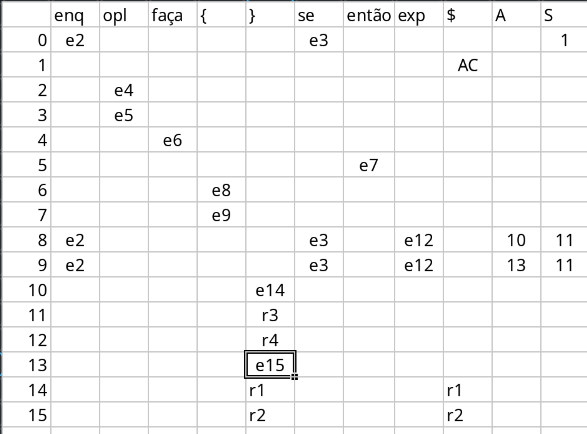
\includegraphics[scale=0.8]{images/tabela-exercicio.png}
\end{document}
\end{document}
